\documentclass{article}

\usepackage[spanish]{babel}
\usepackage[numbers,sort&compress]{natbib}
\usepackage{graphicx}
\usepackage{url}
\usepackage{amsmath}
\usepackage{hyperref}
\usepackage[top=30mm, bottom=40mm, left=15mm, right=15mm]{geometry}
\setlength{\parskip}{2mm}
\setlength{\parindent}{0pt}

\author{Abraham Azael Morales Juárez        1422745}
\title{Movimiento Browniano}
\date{\today}

\begin{document}

\maketitle

\section{Objetivos}
-Examinar de manera sistemática los efectos de la dimensión en la probabilidad de regreso al origen del movimiento Browniano para dimensiones 1 a 8 en incrementos lineales de uno, variando el número de pasos de la caminata como potencias de dos con exponente de 6 a 12 en       incrementos lineales de uno, con 30 repeticiones del experimento para cada combinación. Grafica los resultados en una sola figura con diagramas de caja-bigote o de violin de tal forma que facilite comparar entre combinaciones de parámetros para poder evaluar si afectan los dos  o si uno domina el comportamiento. \url{[1]}

\section{Resultados}
Los datos obtenidos a partir de las corridas virtuales reflejaron, como se puede ver en la Figura 1, distintos escenarios que se pudieron gráficar para una mejor comparación y entendimiento; cada uno de estos con determinadas especificaciones nos mostró que entre mayor sea la cantidad de dimensiones existentes para el movimiento aleatorio de una partícula más lejana de su origen quedara al final de su movimiento. Cada gráfica se corrio 30 veces para poder determinar si por estadística puediera volver al origen. Pero los resultados mostrarón que (almenos con las variables con las que se realizo el estudio) se aleja cada vez más del origen. Sin embargo, no se descarta la posibilidad de que esto pueda ocurrir, se necesitaría realizar otra corrida con diferentes parámetros para poder obtener un resultado positivo.

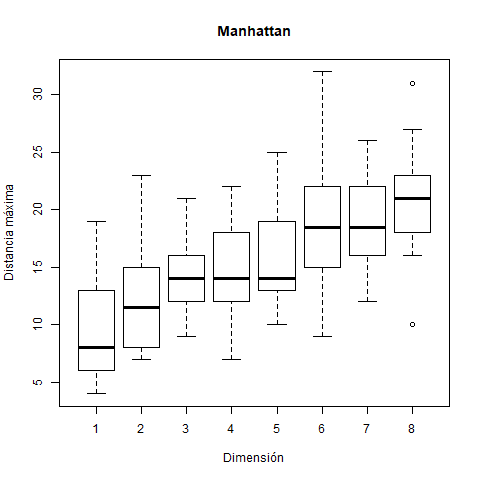
\includegraphics[width=7cm]{../Documents/manganthan2ala6.png}  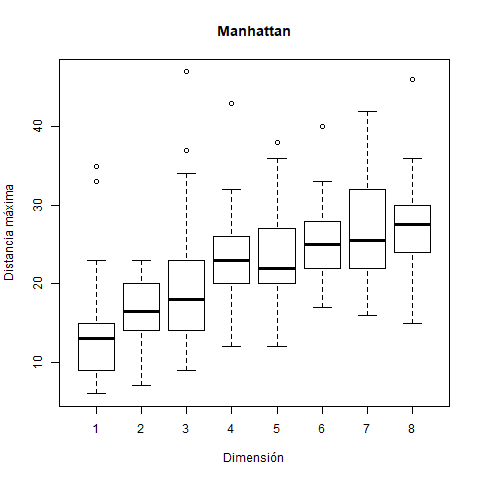
\includegraphics[width=7cm]{../Documents/manganthan2ala7.png} 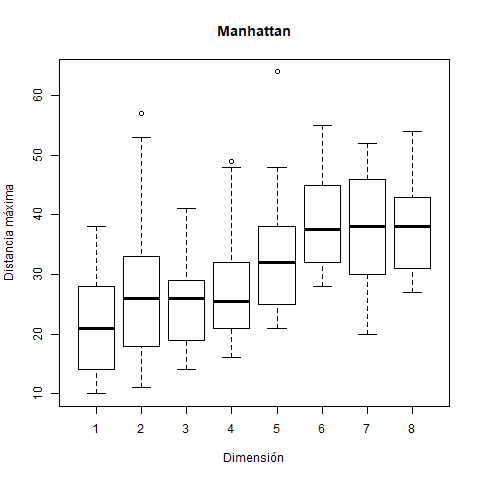
\includegraphics[width=7cm]{../Documents/manganthan2ala8.png} 

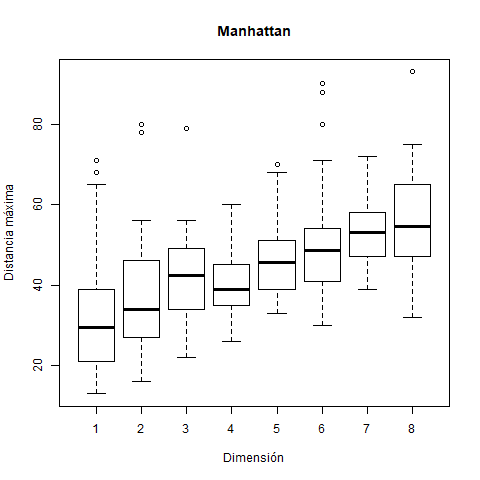
\includegraphics[width=7cm]{../Documents/manganthan2ala9.png} 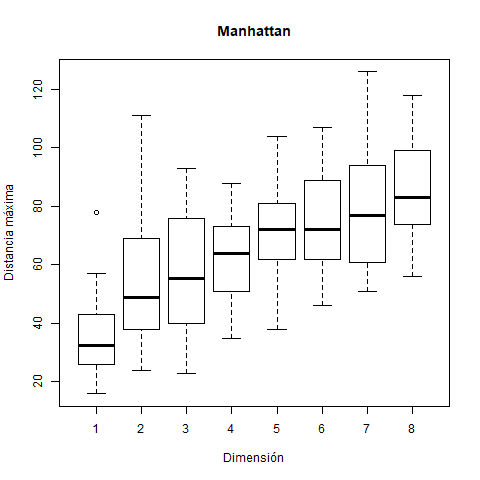
\includegraphics[width=7cm]{../Documents/manganthan2ala10.png} 


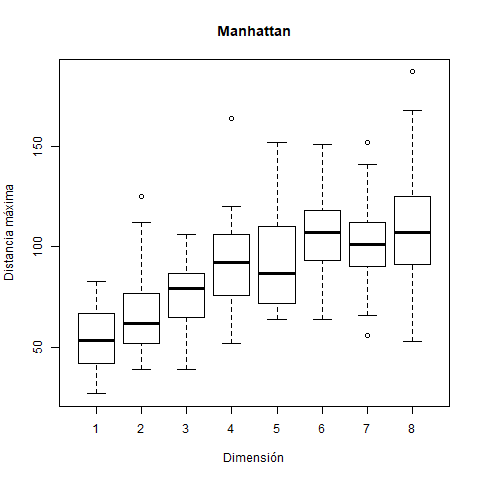
\includegraphics[width=7cm]{../Documents/manganthan2ala11.png}  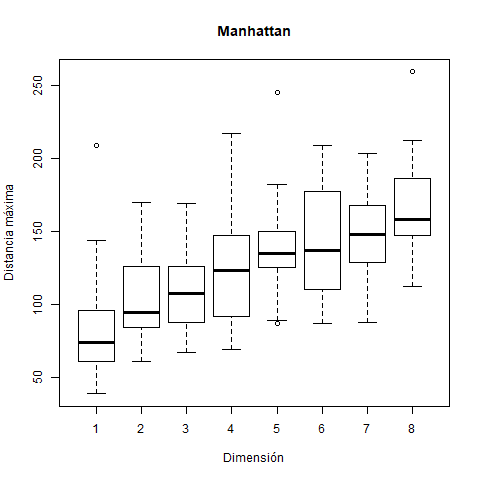
\includegraphics[width=7cm]{../Documents/manganthan2ala12.png} 

{Fig. 1.- Graficas de comparación Manhattan, en orden de 2*6 hasta 2*12}

\section{Conclusiones}
Se pudo concluir que entre máyor cantidad de dimensiones y menor número de pasos, la probabilidad de que una partícula en movimiento aleatorio vuelva al estado inicial es practicamente nula.


\bibliographystyle{plainnat}
\bibliography /{[1] https://elisa.dyndns-web.com/teaching/comp/par/p1.html}


\end{document}